\textbf{Метод 2 --- Кубический сплайн}\\

\textbf{Задание}

Построить кубический сплайн для функции, заданной в узлах интерполяции, предполагая, что сплайн имеет нулевую кривизну при $x=x_0$ и $x=x_4$. Вычислить значение функции в точке $x=X^*$.\\

\textbf{Вариант:} 3

$X^*=1.5$\\
\begin{tabular}{|c|c|c|c|c|c|}
\hline
i & 0 & 1 & 2 & 3 & 4 \\
\hline
$x_i$ & 0.0 & 0.9 & 1.8 & 2.7 & 3.6 \\
\hline
$f_i$ & 0.0 & 0.36892 & 0.85408 & 1.7856 & 6.3138 \\
\hline
\end{tabular}
\vspace{0.5cm}

\textbf{Описание алгоритма}

Наиболее широко применяемым является случай, когда между любыми двумя точками разбиения исходного отрезка строится многочлен $n$--й степени:

$$
S(x)=\sum\limits_{k=0}^na_{ik}x^k, x_{i-1} \leq x \leq x_i, i=1,...,n
$$

который в узлах интерполяции принимает значения аппроксимируемой функции и непрерывен вместе со своими $(n-1)$ производными. Такой кусочно-непрерывный интерполяционный многочлен называется сплайном. Его коэффициенты находятся из условий равенства в узлах сетки значений сплайна и приближаемой функции, а также равенства $n-1$ производных соответствующих многочленов. На практике наиболее часто используется интерполяционный многочлен третьей степени, который удобно представить как:\\

$S(x)=a_i+b_i(x-x_{i-1})+c_i(x-x_{i-1})^2+d_i(x-x_{i-1})^3$\\
$x_{i-1} \leq x \leq x_i, i=1,2,...,n$\\

Для построения кубического сплайна необходимо построить $n$ многочленов третьей степени, т.е. определить $4n$ неизвестных $a_i, b_i, c_i, d_i$. Эти коэффициенты ищутся из условий в узлах сетки.\\

$S(x_{i-1})=a_i=a_{i-1}+b_{i-1}(x_{i-1}-x_{i-2})+c_{i-1}(x_{i-1}-x_{i-2})^2+d_i(x_{i-1}-x_{i-2})^3=f_{i-1}$\\
$S'(x_{i-1})=b_i=b_{i-1}+2c_{i-1}(x_{i-1}-x_{i-2})+3d_{i-1}(x_{i-1}-x_{i-2})^2$\\
$S''(x_{i-1})=2c_i=2c_{i-1}+6d_{i-1}(x_{i-1}-x_{i-2}), i=2,3,...,n$\\
$S(x_0)=a_1=f_0$\\
$S''(x_0)=c_1=0$\\
$S(x_n)=a_n+b_n(x_n-x_{i-1})+c_n(x_n-x_{i-1})^2+d_n(x_n-x_{i-1})^3=f_n$\\
$S''(x_n)=c_n+3d_n(x_n-x_{i-1})=0$\\

Предполагается, что сплайны имеют нулевую кривизну на концах отрезка.

Если ввести обозначение $h_i=x_i-x_{i-1}$, и исключить из системы $a_i, b_i, d_i$, то можно получить систему из $n-1$ линейных алгебраических уравнений относительно $c_i, i=2,...,n$ с трехдиагональной матрицей:\\

$2(h_1+h_2)c_2+h_2c_3=3[(f_2-f_1)/h_2-(f_1-f_0)/h_1]$\\
$h_{i-1}c_{i-1}+2(h_{i-1}+h_i)c_i+h_ic_{i+1}=3[(f_i-f_{i-1})/h_i-(f_{i-1}-f_{i-2})/h_{i-1}], i=3,...,n-1$\\
$h_{n-1}c_{n-1}+2(h_{n-1}+h_n)c_n=3[(f_n-f_{n-1})/h_n-(f_{n-1}-f_{n-2})/h_{n-1}]$\\

Остальные коэффициенты сплайнов могут быть восстановлены по формулам:\\

$a_i=f_{i-1}, i=1,...,n; \quad b_i=(f_i-f_{i-1})/h_i-\frac{1}{3}h_i(c_{i+1}+2c_i), \quad d_i=\frac{c_{i+1}-c_i}{3h_i}, i=1,...,n-1$\\
$c_1=0, b_n=(f_n-f_{n-1})/h_n-\frac{2}{3}h_nc_n, d_n=-\frac{c_n}{3h_n}$\\

\textbf{Реализация}
\begin{lstlisting}
#include "./dependens/TSolve.h"
#include <map>
#include <utility>

using namespace std;

static const size_t powerSplane = 3;

struct TData {
	pair<double, double> pSection;
	vector<double> vKoef;
};

int main(int argc, char* argv[]) {
	if (argc != 2) {
		cerr << "Error: count of args is incorrect" << endl;
		exit(-1);
	}	
	string dataFile = argv[1];
	ifstream in(dataFile, ios::in);

	size_t N;
	vector<double> X, Y;
	vector<TData> table;
	double perfectX;
	double temp;
		
	in >> N;
	for (size_t i = 0; i < N; ++i) {
		in >> temp;
		X.push_back(temp);	
	}
	for (size_t i = 0; i < N; ++i) {
		in >> temp;
		Y.push_back(temp);	
	}
	in >> perfectX;
	in.close();	

	for (size_t i = 1; i < N; ++i) {
		TData temp;
		temp.pSection = make_pair(X[i - 1], X[i]);
		table.push_back(temp);
	}

	string inputFile 	= "./dependens/inputData";
	string outputFile 	= "./dependens/outputData";

	ofstream out(inputFile, ios::out);
	N--;	
	out << N - 1 << endl;
	out << 2 * (X[2] - X[0]) << " " << (X[2] - X[1]) << " " << 0.0 << " " << 3 * ((Y[2] - Y[1]) / (X[2] - X[1]) - (Y[1] - Y[0]) / (X[1] - X[0])) << endl;
	for (size_t i = 3; i <= N - 1; ++i) {
		out << (X[i - 1] - X[i - 2]) << " " << 2 * (X[i] - X[i - 2]) << " " << (X[i] - X[i - 1]) << " " << 3 * ((Y[i] - Y[i - 1]) / (X[i] - X[i - 1]) - (Y[i - 1] - Y[i - 2]) / (X[i - 1] - X[i - 2])) << endl;
	}
	out << (X[N - 1] - X[N - 2]) << " " << 2 * (X[N] - X[N - 2]) << " " << 0.0 << " " << 3 * ((Y[N] - Y[N - 1]) / (X[N] - X[N - 1]) - (Y[N - 1] - Y[N - 2]) / (X[N - 1] - X[N - 2])) << endl;
	out.close();
	TSolve sol(inputFile, outputFile);
	if (!!sol.ToSolveByTripleDiagMatrix()) {
		cerr << "Error: Troubles with method TripleDiagMatrix!" << endl;
		exit(-1);
	}
	in.close();
	in.open(outputFile);
	vector<double> vecC;
	vecC.push_back(0.0);
	while (in >> temp) {
		vecC.push_back(temp);
	}
	in.close();
	for (size_t i = 1; i < N; ++i) {
		vector<double> t(powerSplane + 1);
		t[0] = Y[i - 1];
		t[1] = (Y[i] - Y[i - 1]) / (X[i] - X[i - 1]) - 1.0 / 3 * (X[i] - X[i - 1]) * (vecC[i] + 2 * vecC[i - 1]);
		t[2] = vecC[i - 1];
		t[3] = (vecC[i] - vecC[i - 1]) / (3 * (X[i] - X[i - 1]));
		table[i - 1].vKoef = t;	
 	}
 	vector<double> vecTemp;
 	vecTemp.push_back(Y[N - 1]);
 	vecTemp.push_back((Y[N] - Y[N - 1]) / (X[N] - X[N - 1]) - 2.0 / 3 * (X[N] - X[N - 1]) * vecC[N - 1]);
 	vecTemp.push_back(vecC[N - 1]);
 	vecTemp.push_back(-vecC[N - 1] / (3 * (X[N] - X[N - 1])));
 	table[N - 1].vKoef = vecTemp;
	// draw graphics
	double deltaX = 0.01;	
	for (size_t i = 0; i < table.size(); ++i) {
		double start = table[i].pSection.first;
		double end = table[i].pSection.second;
		ofstream out("plotData" + to_string(i), ios::out);
		for (double cur = start; cur <= end; cur += deltaX) {
			double f = .0;
			for (size_t k = 0; k < table[i].vKoef.size(); ++k) {
				f += table[i].vKoef[k] * pow(cur - start, k * 1.0);
			}
			out << cur << " " << f << endl;
		}
		cout << "[" << table[i].pSection.first << "; " << table[i].pSection.second << "]\t";
		for (size_t j = 0; j < table[i].vKoef.size(); ++j)
			cout << table[i].vKoef[j] << " ";
		cout << endl;
	}	
	return 0;
}
\end{lstlisting}
\vspace{0.5cm}

\textbf{Тестирование}\\

\textbf{Входной файл}
\begin{verbatim}
5
0.0 0.9 1.8 2.7 3.6
0.0 0.36892 0.85408 1.7856 6.3138
1.5
\end{verbatim}

\textbf{Выходной файл}
\begin{verbatim}
[0; 0.9]		0 			0.339411 	0 		0.087037 
[0.9; 1.8]	0.36892 		0.551067 	0.235 	-0.275926 
[1.8; 2.7]	0.85408 		0.303022 	-0.51 	1.47037 
[2.7; 3.6]	1.7856 		2.95533 		3.46 	-1.28148
\end{verbatim}

\textbf{График}

\begin{center}
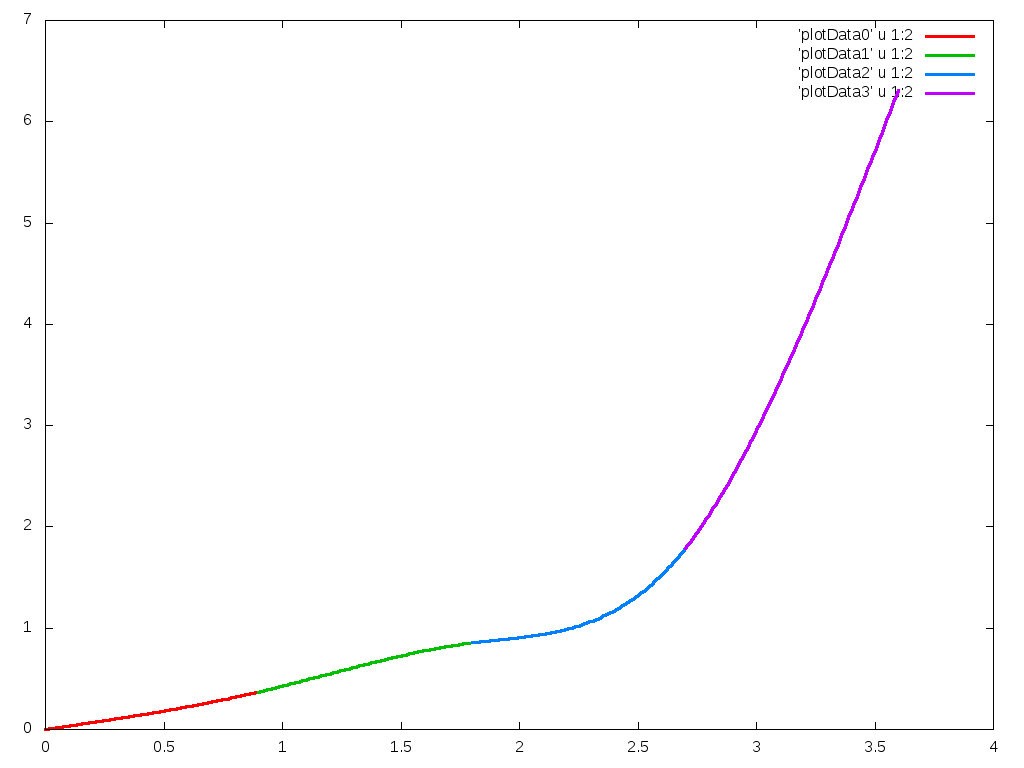
\includegraphics[scale=0.5]{images/graphic3_2.png}
\end{center}

\pagebreak
